\documentclass[a4paper,10pt]{article}

\usepackage[english,activeacute]{babel}
\usepackage[english]{layout}
\usepackage{amsfonts,amsmath,amssymb,amsthm}
\usepackage[dvips]{graphicx}
\usepackage{color}
\usepackage{subfig}
\usepackage{colonequals}
\usepackage[latin1]{inputenc}
\usepackage{url}
\usepackage{epsfig}
\usepackage{dsfont}

\usepackage{algorithm}
\usepackage{algorithmic}
\usepackage{setspace}
\usepackage{afterpage}
%\usepackage{showkeys}
% \usepackage{mathptmx}      % use Times fonts if available on your TeX system
% \usepackage{latexsym}

%\usepackage[left=1.2in,right=1.2in]{geometry}

% \graphicspath{{../iccv09/}}

\newcommand{\ma}[1]{\boldsymbol{#1}}
\newcommand{\tras}[1]{#1^{\mathrm{T}}}
\newcommand{\herm}[1]{#1^{\mathrm{H}}}
\newcommand{\con}[1]{#1^{\mathrm{*}}}
\newcommand{\E}{\mathds{E}}
\newcommand{\tech}[1]{\overline{#1}}
\newcommand{\nspace}{\!\!\!\!}
\newcommand{\nmbr}[1]{\oldstylenums{#1}}

\newcommand{\eg}{\emph{e.g}. } \newcommand{\Eg}{\emph{E.g}. }
\newcommand{\ie}{\emph{i.e}. } \newcommand{\Ie}{\emph{I.e}. }
\newcommand{\cf}{\emph{c.f}. } \newcommand{\Cf}{\emph{C.f}. }
\newcommand{\etc}{\emph{etc}. } \newcommand{\vs}{\emph{vs}. }
\newcommand{\wrt}{w.r.t\onedot } \newcommand{\dof}{d.o.f. }
\newcommand{\etal}{\emph{et al}. }

\newcommand{\R}{\mathds{R}}
\newcommand{\sign}{\mathrm{sign}}
\newcommand{\eps}{\varepsilon}
\newcommand{\To}{\longrightarrow}
% \newcommand{\II}{1{\hskip -2.5 pt}\hbox{I}}

% c++ code
\usepackage{listings}
\usepackage{xcolor}
\usepackage{textcomp}
\definecolor{listinggray}{gray}{0.9}
\definecolor{lbcolor}{rgb}{0.9,0.9,0.9}
\lstset{
	backgroundcolor=\color{lbcolor},
	tabsize=4,    
%  rulecolor=,
	language=Matlab,
	basicstyle=\scriptsize\ttfamily,
	upquote=true,
	aboveskip={1.5\baselineskip},
	columns=fixed,
	showstringspaces=false,
	extendedchars=false,
	breaklines=true,
	prebreak = \raisebox{0ex}[0ex][0ex]{\ensuremath{\hookleftarrow}},
	frame=single,
	numbers=left,
	showtabs=false,
	showspaces=false,
	showstringspaces=false,
	identifierstyle=\ttfamily,
	keywordstyle=\color[rgb]{0,0,1}\ttfamily,
	commentstyle=\color[rgb]{0,0.5,0}\ttfamily,
	stringstyle=\color[rgb]{0.627,0.126,0.941}\ttfamily,
	numberstyle=\color[rgb]{0.5, 0.5, 0.5}\ttfamily,
%  \lstdefinestyle{C++}{language=C++,style=numbers}’.
}
%\lstset{
%	backgroundcolor=\color{lbcolor},
%	tabsize=4,
%	language=C++,
%	captionpos=b,
%	tabsize=3,
%	frame=lines,
%	numbers=left,
%	numberstyle=\tiny,
%	numbersep=5pt,
%	breaklines=true,
%	showstringspaces=false,
%	basicstyle=\footnotesize,
%	identifierstyle=\color{magenta},
%	keywordstyle=\color[rgb]{0,0,1},
%	commentstyle=\color{green},
%	stringstyle=\color{red}
%}
	
	
	


\DeclareMathOperator*{\argmin}{arg\,min}
\DeclareMathOperator*{\argmax}{arg\,max}

\newcommand{\nota}[1]{\textcolor{blue}{\textbf{#1}}}
\newcommand{\suggest}[1]{\textcolor{yellow}{#1}}
\newcommand{\add}[1]{\textcolor{green}{#1}}
\newcommand{\remove}[1]{\textcolor{red}{#1}}
\newcommand{\dosdv}[1] {#1}
\newcommand{\uncite}[1] {}
% \newcommand{\tachar}[1]{
% \setbox4=\hbox{\ } \setbox3=\hbox{#1} \hbox{#1} \kern -\wd3 \kern
% -\wd4 \raise 0.3\ht3 \hbox{ \vrule width \wd3 height 0.5pt} }

% \theoremstyle{plain}\newtheorem{theorem}{Theorem}[chapter]
% \theoremstyle{plain}\newtheorem{proposition}{Proposition}[chapter]
% \theoremstyle{plain}\newtheorem{lemma}{Lemma}[chapter]
% \theoremstyle{definition}\newtheorem{definition}{Definition}[chapter]

\title{Aggregation of empirical Wiener estimates}
\author{}
\date{}

\begin{document}

\maketitle

\section{Setting}

\paragraph{Signal.}We assume a very simple setting. Suppose we have $N$ signals in $\mathbb R^d$,
assumed to follow a Gaussian distribution
\[x_i\sim \mathcal N(0,\Lambda), \quad i\in1,\dots,N.\]
where $\Lambda =
\text{diag}(\lambda_1,\lambda_2,\dots,\lambda_d)$.

\paragraph{Observations.}We have $M$ observations of these signals, contaminated
by additive white Gaussian noise:
\[y_{ij} = x_i + n_{ij}, \quad i = 1,\dots,N, j = 1,\dots,M,\]
where $n_{ij}\sim \mathcal N(0,\sigma^2I)$.
These observations are not available simultaneously, but sequentially in $M$ batches.

\paragraph{Wiener filter.}For each of the $M$ groups of observations, we compute an empirical Wiener
estimate of the signals $x_i$:
\[\hat x_{ij} = \widehat W_jy_{ij} = \widehat W_j x_i + \widehat W_j n_{ij}.\]
The coefficients of the Wiener filter are estimated from the group of $N$ observations
available at time $j$:
\[\hat w_j(k) = \frac{\hat \lambda_k}{\hat \lambda_k + \sigma^2} =
\frac{\frac1N \sum_{i = 1}^N y_{ij}(k)^2 -\sigma^2}{\frac1N \sum_{i = 1}^N y_{ij}(k)^2} = 
1 - \sigma^2\left(\frac1N\sum_{i = 1}^N y_{ij}(k)^2\right)^{-1}.\]
Alternatively, we also defined the thresholded empirical Wiener filter
as 
\[\hat w_j^+(k) = \hat w_j(k) \cdot \frac12 (\text{sign}(\hat w_j(k)) + 1).\]

\paragraph{Aggregation.}The final estimate is done by aggregating the $M$
Wiener estimates:
\[\hat x_i = \frac1M \sum_{j = 1}^M \hat x_{ij} = x_i \frac1M \sum_{j = 1}^M
\widehat W_j + \frac1M \sum_{j = 1}^M \widehat W_jn_{ij}\]

\paragraph{Aim.}The aim is to evaluate the performance of $\hat w_j$ and $\hat
w_j^+$. For that sake, we will compute the PDF of $\hat w_j(k)$, and the PDF of the
aggregated weights. If $M$ is large, we can approximate the aggregation by an 
expectation:
\[\hat x_i(k)\to \mathbb E\{ \hat w_j(k) \} x_i(k) + \mathbb E\{w_j(k) n_{ij}(k)\}\]
where the expectation is taken over variables $n_{1j}(k), \dots, n_{Nj}(k)$,
for each $i, k$. Similarly for the thresholded coefficients.

\section{PDF of filter coefficients}

Let us for now focus on the non-thresholded filter coefficients 
\[\hat w_j(k) =  
1 - \sigma^2\left(\frac1N\sum_{i = 1}^N y_{ij}(k)^2\right)^{-1}.\]
The variance of $y_{ij}(k)$ follows a non-central chi squared distribution,
and therefore $\hat w_j(k)$ corresponds to a random variable which is the
reciprocal of a non-central chi squared distribution. 

\subsection{The variance along dimension $k$}

Let us include the following notation for the variance of the observations
along dimension $k$
\[v_j(k) = \frac1N\sum_{i = 1}^Ny_{ij}(k)^2.\]

\paragraph{Scaled non-central $\chi^2$.}Let us consider
$\nu = a\sum_{i = 1}^N (\mu_i + \xi_i)^2$, where $a, N$ and $\mu_i$, $i =
1,\dots,N$ are known parameters and $\xi\sim\mathcal N(0,1)$. 
Then, $\nu$ follows a scaled non-central chi-squared distribution,
$\nu\sim\chi^2_N(\mu,a)$, where
\[\mu = \sum_{i = 1}^N \mu_i^2\]
is called the non-centrality parameter.
The PDF has the following expression:
\[f(\nu; N, \mu, a) = \frac1{2|a|} e^{-(\nu/a+\mu)/2}\left(\frac{\nu}{a\mu}\right)^{N/4 - 1/2} I_{N/2-1}(\sqrt{\mu\nu/a}),\]
where $I_{N/2-1}$ is a modified Bessel function of the first kind,
\[I_r(z) = (z/2)^r\sum_{i = 0}^\infty\frac{(z^2/4)^i}{i!\Gamma(r + i + 1)},\]
where the gamma function is a real extension of the factorial 
given by 
\[\Gamma(t) = \int_0^\infty x^{t-1}e^{-x}dx.\]
It has the property that $\Gamma(i) = (i-1)!$ for $j\in\mathbb N_+$.
The mean and variance of this distribution are given by
\[\mathbb E\{\nu\} = a(N + \mu)\quad\quad\mathbb V\{\nu\} = 2a^2(N + 2\mu).\]

\paragraph{The distribution of $v_j(k)$.}By scaling the terms in the summation
to normalize the variance, we have that 
\[v_j(k)\sim \chi^2_N\left(\frac1{\sigma^2}\sum_{i = 1}^Nx_i^2(k), \frac{\sigma^2}N\right) = \chi^2_N\left(N\hat{\text{snr}}(k), \frac{\sigma^2}N\right),\]
where we have defined 
\[\hat{\text{snr}}(k) = \frac1{N\sigma^2}\sum_{i = 1}^Nx_i^2(k).\]
Note that this ``sample signal-to-noise ratio'' cannot be computed in practice, since
it requires the knowledge of the $x_i$. It can be seen as an approximation of the
true signal to noise ratio $\lambda_k/\sigma^2$, specially for $N$ large.

The mean and variance of the sample variance are then
\begin{align*}
\mathbb E\{v_j(k)\} &= \sigma^2 + \frac1N\sum_{i = 1}^N x_i^2(k) =  \sigma^2(1 + \hat{\text{snr}}(k)),\\
\mathbb V\{v_j(k)\} &= \frac{2\sigma^2}N\left(\sigma^2 + \frac2N \sum_{i =1}^N x_i^2(k)\right) = \frac{2\sigma^4}N\left(1 + 2\hat{\text{snr}}(k)\right).
\end{align*}

\paragraph{Gaussian approximation.}In the limit when $N$ or $\mu$ tend to infinity, this distribution converges to
a Gaussian with the same mean and variance. The Gaussian approximation is valid in
our setting, since both $N$ and $\mu$ are large. 

\subsection{The reciprocal of a scaled non-central chi squared}

If $\xi$ is a random variable with PDF $f$ supported in the positive axis, then
the PDF of $\nu = 1/\xi$ is $g$ given by
\[g(\nu) = 1/{\nu^2}f(1/\nu).\]
Furthermore, if $\zeta = 1 - b\nu = 1 - b/\xi$ with $b>0$, then its PDF $h$ is
given by: 
\[h(\zeta) = \frac1b g((1 - \zeta)/b) = \frac b{(1-\zeta)^2}f(b/(1-\zeta) ).\]

We have that $\hat w_j(k) = 1 - \sigma^2/v_j(k)$, thus we can obtain the PDF of the 
filter coefficient using the previous relationship for $f$ the PDF of scaled non-central
chi squared and $b = \sigma^2$. The resulting PDF has the following expression:
\begin{multline*}
	h(\omega) = \frac{N}{2(1 - \omega)^2}
\exp\left(-\frac12\left[\frac{N}{(1-\omega)} + \frac1{\sigma^2}\sum_{i=1}^Nx_i^2(k)\right]\right)\\
\left(\frac{N\sigma^2}{(1-\omega)\sum_{i = 1}^N x_i^2(k)}\right)^{N/4-1/2}
I_{N/2-1}\left(\sqrt{\frac{N}{\sigma^2(1 - \omega)}\sum_{i =
1}^Nx_i^2(k)}\right)
\end{multline*}
Or equivalently:
\begin{multline*}
	h(\omega) = \frac{N}{2(1 - \omega)^2}
	\exp\left(-\frac{N}{2}\left[\frac{1}{(1-\omega)} + \hat{\text{snr}}(k)\right]\right)\\
	\left(\frac{1}{(1-\omega)\hat{\text{snr}}(k)}\right)^{N/4-1/2}
	I_{N/2-1}\left(\sqrt{\frac{N^2}{(1 - \omega)}\hat{\text{snr}}(k)}\right)
\end{multline*}

\noindent\textcolor{red}{Is there a closed form expression for the mean and variance of this distribution?}

The weights are obtained by applying a concave function $\varphi(v) = 1 -
\sigma^2/v$, to the sample variance $v$. From Jensen's inequality, we know that
\[\mathbb E\{\hat w_j(k)\} = \mathbb E\{\varphi(v_j)\} < \varphi(\mathbb
E\{v_j\}) = 1 - \frac{1}{1 + \hat{\text{snr}}(k)}.\]

\noindent\textcolor{red}{Are there similar results bounding the variance?}

\paragraph{Gaussian approximation.}When the empirical variance can be approximated by a Gaussian, 
and its support is small compared with the concavity of $\varphi$, such that $\varphi$ can be 
assumed to be linear, then the weights are approximately Gaussian distributed. In this case,
we have that
\[\mathbb E\{\hat w_j(k)\}\approx \varphi(\mathbb E\{v_j\}) =\frac{\hat{\text{snr}}(k)}{1 + \hat{\text{snr}}(k)},\]
and that
\[\mathbb V\{\hat w_j(k)\}\approx \varphi'(\mathbb E\{v_j\})^2 \mathbb V\{v_j\}=
\frac{2}N\frac{\left(1 + 2\hat{\text{snr}}(k)\right)}{(1 + \hat{\text{snr}}(k))^4}.\]
For this Gaussian approximation to be valid, we need $N$ and/or
$\hat{\text{snr}}(k)$ to be large enough. The number of samples $N$ has the effect of 
reducing the support of the distribution, where increasing $\hat{\text{snr}}$ shifts the
distribution towards larger values of $v$, where $\varphi$ has less curvature.

\begin{figure}[htpb!]
	\centering
	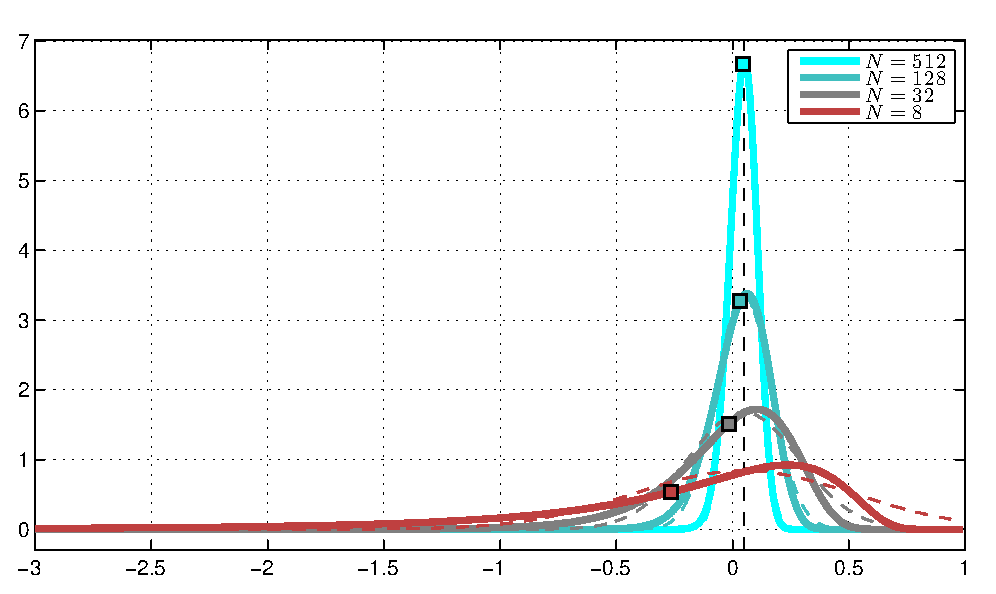
\includegraphics[width=0.9\textwidth]{weight_pdf}
	\caption{PDF of the Wiener coefficients, varying $N$, for a SNR of 0.1. The mean of each PDF
	is shown as a square on the graph. The Gaussian approximations are shown as
	the dashed curves. The dashed vertical line indicates $\varphi(\mathbb E\{v_j\})$.}
	\label{fig:wiener_pdf_N}
\end{figure}

\begin{figure}[htpb!]
	\centering
	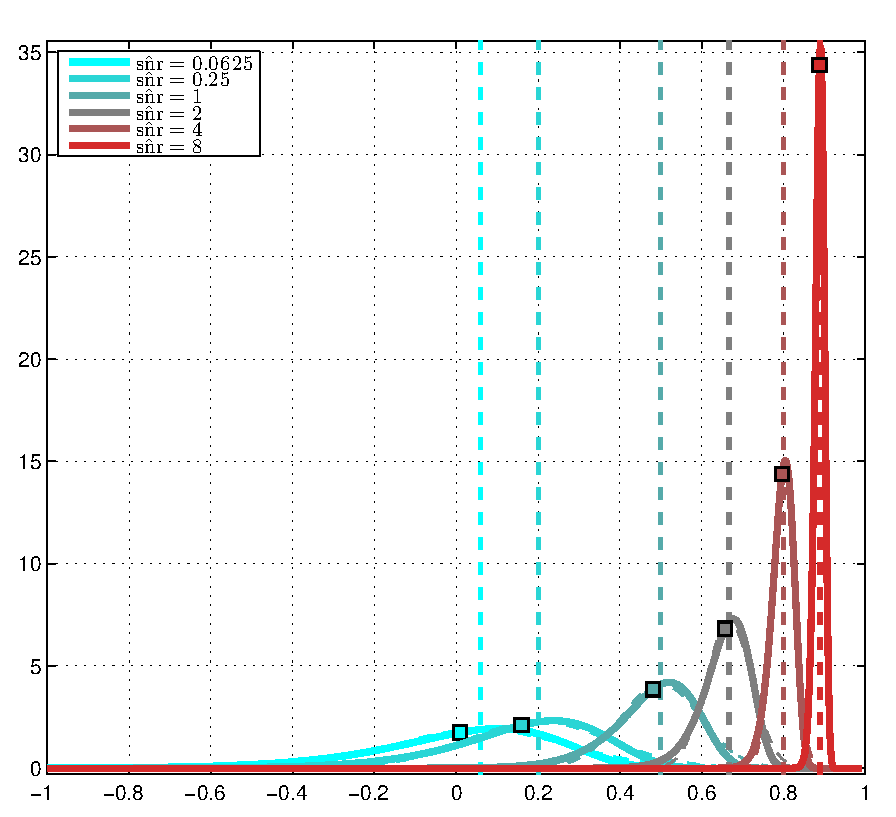
\includegraphics[width=0.9\textwidth]{weight_pdf-snr}
	\caption{PDF of the Wiener coefficients, varying $\hat{\text{snr}}$, for $N = 40$. The mean of each PDF
	is shown as a square on the graph. The Gaussian approximations are shown as
	the dashed curves. The dashed vertical lines indicate $\varphi(\mathbb E\{v_j\})$.}
	\label{fig:wiener_pdf_N}
\end{figure}

\section{Wiener estimates of the signal}

In the preceding sections we derived the PDF of
the weights of the empirical Wiener filter.
In the present section we will study the Wiener estimates of the signals $x_i$.

\subsection{Single Wiener estimate}

The Wiener estimate is given by
\[\hat x_{ij}(k) = \hat w_j(k) x_i(k) + \hat w_j(k)n_{ij}(k).\]
We consider that the $x_i$ are fixed, and study the effect of the noise.

As we have seen in the previous section, the filter coefficient is a random
variable depending on the noise (also on the sampled signals $x_i$, but we
are considering them fixed). The Wiener estimate $\hat x_{ij}(k)$ is given
by a product of random variables. Let us open a parenthesis to discuss the
PDF of a product of two random variables.

\paragraph{The PDF of a product of random variables.}
For two random variables $X,Y$, let $Z = XY$. The PDF of $Z$ can be computed as
\[f_Z(z) = \int_{-\infty}^{\infty} f_X(x)f_Y(z/x)\frac1{|x|}d x.\]
In our case, it seems difficult to derive a closed-form expression for the PDF
of the Wiener estimate, even if we adopt a Gaussian approximation. In the case
in which $X,Y$ are Gaussian, the distribution of the product is given by a 
linear combination of non-central chi squared random variables. This follows
from the following decomposition:
\[XY = \frac14(X + Y)^2 - \frac14(X-Y)^2.\]
Both terms are squared Gaussian random variables, and thus follow a non-central
chi squared distribution. Note also, that except if $X,Y$ have the same variance,
$X+Y$ and $X-Y$ are not independent. In this case, to compute the distribution of
the sum we require the joint distribution of $(X+Y)^2$ and $(X-Y)^2$.


%The first term is a scaling of the filter coefficient. For the second term
%we will adopt the simplifying assumption that the weight and the noise are
%independent. This is a valid approximation when $N$ is large, but becomes
%less valid when $N$ is small and $\sigma$ large, since each each realization 
%of the noise has a greater impact on the weight. The assumption of independence
%can be interpreted as if the weights were estimated using a realization of the
%noise, and then used to filter an additional independent realization.
%
%For the product of two random variables $Z = XY$, we have that
%\[XY = e^{\log X + \log Y},\]
%thus, computing the product amounts to applying a logarithm to both PDFs,
%convolving them, and applying an exponential to the result.
%The problem here is that our random variables can take negative values,
%invalidating this approach. If we assume that the weights follow a 
%Gaussian distribution, then we can express the distribution of the
%product as a linear combination of (dependent) chi squared random variables,
%because of the following relation:
%Except $X$ and $Y$ have same variance, both terms are dependent. 

Instead of computing the PDF, we can compute its first and second order
moments. If we assume that $X,Y$ are independent, we have that
$\mathbb E\{XY\} = \mathbb E\{X\}\mathbb E\{Y\}$.
The variance could be computed from this equation:
\[\mathbb V\{XY\} = \mathbb E\{X^2Y^2\} - \mathbb E\{XY\}^2 = 
\mathbb V\{X\}\mathbb V\{Y\} +\mathbb V\{X\}\mathbb E\{Y\}^2 + \mathbb E\{X\}^2\mathbb V\{Y\}.\]

In our case, this amounts to
\begin{align*}
	\mathbb E\{\hat x_{ij}(k)\} &= \mathbb E\{\hat w_j(k)\}x_i(k) = \frac{\hat{\text{snr}}(k)}{1 + \hat{\text{snr}}(k)}x_i(k).\\
	\mathbb V\{\hat x_{ij}(k)\} &=  
(x_i(k)^2 + \sigma^2)
\frac{2}N\frac{\left(1 + 2\hat{\text{snr}}(k)\right)}{(1 + \hat{\text{snr}}(k))^4} + 
\sigma^2\frac{\hat{\text{snr}}(k)^2}{(1 + \hat{\text{snr}}(k))^2}.
Y\end{align*}

We can compute the bias:
\begin{multline*}
\mathbb B\{\hat x_{ij}(k)\} = \mathbb E\{\hat x_{ij}(k)-x_i(k)\} \\
= \mathbb E\{\hat w_j(k) x_i(k) - w(k)x_i(k) + w(k)x_i(k) - x_i(k)\}\\
= x_i(k)([\mathbb E\{\hat w_j(k)\} - w(k)] + [w(k) - 1])
\end{multline*}
Thus, we can decompose the bias in two terms. The first one represents the
bias between the empirical Wiener coefficient and the true Wiener coefficient.
Recall that we have that
\[\mathbb E\{\hat w_j(k)\} < \frac{\hat{\text{snr}}(k)}{1 + \hat{\text{snr}}(k)} \xrightarrow{N\to\infty} w(k).\]
The second term corresponds to the bias of the true Wiener filter, and
can be interpreted as the signal components unrecoverable from the noise.

\paragraph{Average squared bias and variance.} We can now compute the
average over the $N$ data points of the variance and the squared bias.
These quantities determine the mean squared error of the estimates.
\begin{align*}
	\frac1N\sum_{i = 1}^N\mathbb B\{\hat x_{ij}(k)\} &= \sigma^2\frac{\hat{\text{snr}}(k)}{(1 + \hat{\text{snr}}(k))^2}.\\
	\frac1N\sum_{i = 1}^N\mathbb V\{\hat x_{ij}(k)\} &=  
\sigma^2\left(\frac{2}N\frac{1 + 2\hat{\text{snr}}(k)}{(1 + \hat{\text{snr}}(k))^3} + 
\frac{\hat{\text{snr}}(k)^2}{(1 + \hat{\text{snr}}(k))^2}\right).
\end{align*}


\subsection{Aggregation of Wiener estimates}

Since we are assuming that the batches of $N$ observations are independent, 
the aggregation of $M$ Wiener estimates maintains the bias, and reduces
the variance by a factor of $M$.
%
%Thus we have that:
%\begin{align*}
%	\mathbb E\left\{\hat x_i(k)\right\} &= \frac{\hat{\text{snr}}(k)}{1 + \hat{\text{snr}}(k)}x_i(k).\\
%	\mathbb V\left\{\hat x_i(k)\right\} &=  
%(x_i(k)^2 + \sigma^2)
%\frac{2}{MN}\frac{\left(1 + 2\hat{\text{snr}}(k)\right)}{(1 + \hat{\text{snr}}(k))^4} + 
%\frac{\sigma^2}{M}\frac{\hat{\text{snr}}(k)^2}{(1 + \hat{\text{snr}}(k))^2}.
%\end{align*}
%
The aggregation attenuates the variance, but does not eliminate the bias. The bias
comes from two sources (i) we are estimating the Wiener coefficients using in every
batch the same $N$ signals, (ii) the bias of the true Wiener filter. The
resulting mean squared error is largely dominated by the bias when $M$ is large.


\paragraph{Comparison with the sample mean.}Note that in this particular
setting (having $M$ noisy versions of the same $N$
signals), a reasonable estimator is just
\[\check x_i = \frac1M\sum_{j = 1}^M y_{ij}(k).\]
This estimate is unbiased, and has a variance of $\sigma^2/M$.

From the expression of the $\mathbb V\{\hat x_{ij}\}$, it can be verified that for $N > 2$, 
\[\frac1N\mathbb V\{\hat x_i(k)\} = \frac1{MN}\sum_{i = 1}^N\mathbb V\{\hat
x_{ij}(k)\} < \sigma^2/M.\]
For $N = 2$ the equality can be achieved if
$\hat{\text{snr}}(k) = 0$. Therefore the variance of the aggregated Wiener estimates
is never larger than the variance of the sample mean. However, the bias is much
larger than $\sigma^2/M$, except for very small values of $M$.
As a consequence, the sample mean has a smaller mean square error already for
moderate values of $M$.


\subsection{The effect of thresholding}

If we consider that $M$ is large enough, we can neglect the variance,
and we can analyze the effect of thresholding in the bias.
The thresholding becomes relevant for components $k$ with a small 
signal energy. These components have already a considerable bias
due the damping of the Wiener filter, which causes signal loss.

We can analyze the first component of the bias, given by
\[b_1(\hat x_{ij}) = x_i(k)(\mathbb E\{\hat w_j(k)\} - w(k)).\]
On one hand, we have that
\[\mathbb E\{\hat w_j(k)\} < \mathbb E\{\hat w^+_j(k)\}.\]
On the other hand we have that
\[\mathbb E\{\hat w_j(k)\} < \frac{\hat{\text{snr}}(k)}{1 + \hat{\text{snr}}(k)} \xrightarrow{N\to\infty} w(k).\]
Therefore it is not easy to see a priori if the effect of the thresholding is 
negative or positive, by compensating the effect of the concave transformation.

In any case, if we consider the full bias, it seems that thresholding should be
in general positive, since it makes the filter coefficient closer to one.






\section{An experimental verification}

We perform a simple numerical simulation to verify the derivations above.
We generate $N$ random vectors in $\mathbb R^d$, with $d = 100$. These 
vectors are generated from a normal distribution given by
\[x_i\sim \mathcal N(0, 4\cdot\text{diag}[(d-1)^2,(d-2)^2,\dots,1,0]).\]
For each of the $N$ vectors, we generate $M$ noisy observations with $\sigma =
20$, and we compute $M$ empirical Wiener estimates, with and without thresholding, $\hat
x^+_{ij}$ and $\hat x_{ij}$.

\begin{figure}[htpb!]
	\centering
	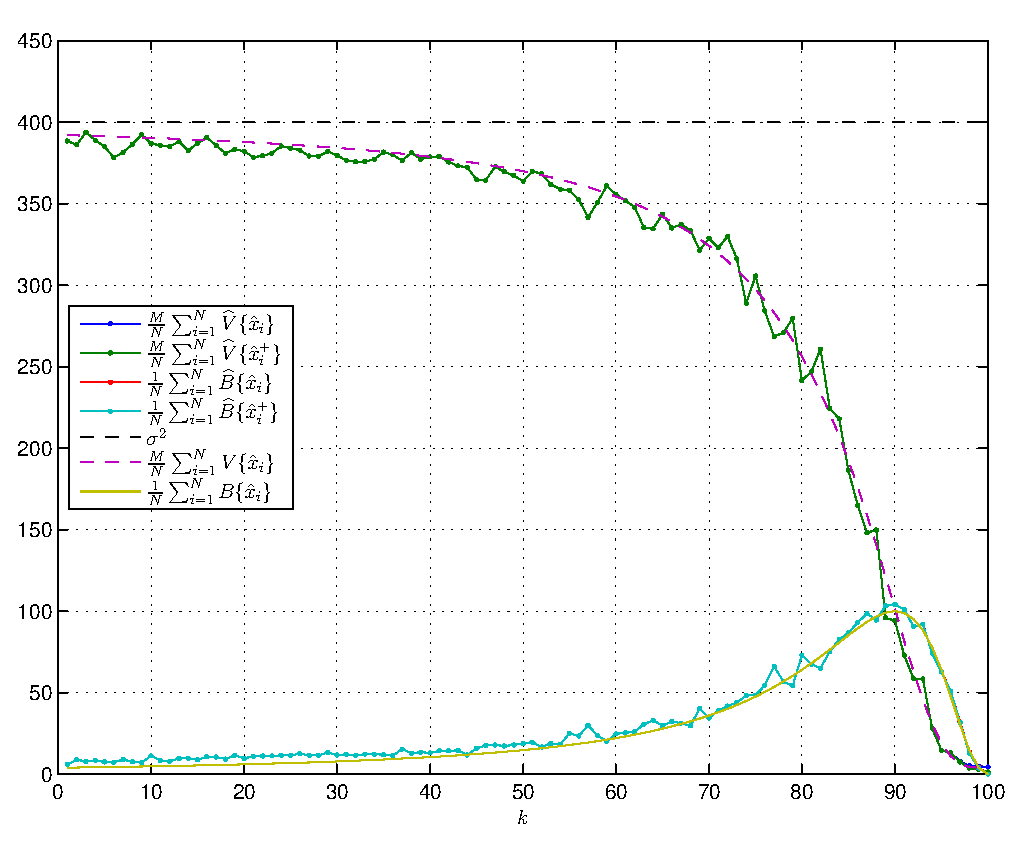
\includegraphics[width=.9\textwidth]{variance-bias}
	\caption{Squared bias and variances averaged over the $N$ points $x_i$. The variances
	correspond to the single Wiener estimate (\ie the variances after aggregation should
	be divided by $M$). The theoretical squared bias and variance and also shown
	for comparison. The variation with the component index $k$ reflects the fact that 
	each component has different signal-to-noise ratio.}
	\label{fig:bias-variance}
\end{figure}

We perform an experiment setting $N = 200$ and $M = 100$. To validate the above
derivations, we compute the empirical variance and squared bias of the single Wiener
estimates as follows:
\begin{align*}
\widehat V\{\hat x_i(k)\} &= \frac1M \sum_{j=1}^M(\hat x_{ij}(k) - \hat x_i(k))^2\\
\widehat B\{\hat x_i(k)\} &= \frac1M \sum_{j=1}^M(\hat x_{ij}(k) - x_i(k))^2 - \widehat V\{\hat x_i(k)\}
\end{align*}
Figure \ref{fig:bias-variance} plots the empirical variances and squared bias,
averaged over the $N$ vectors $x_i$ as a function of the component index $k$.
The results are shown for the thresholded and unthresholded versions of the
filter (the plots are almost identical).
We also show the theoretical variance and bias, computed from the formulas
derived above.
The variances in the plot correspond to the sigle Wiener estimate. 
Note how the variances are bellow $\sigma^2$, as predicted.
After aggregation,
this variances are reduced by a factor of $M$.
The bias however, does not change, which causes the sample mean to perform better.
In the present example the RMSE was $5.51$ for both versions of the Wiener filter,
and $1.99$ for the sample mean.

It can be oversved a slight better performance of the thresholded filter. The reason,
as discussed above, is that thresholding creates a bias for the small Wiener
weights, making them larger. This reduces the bias of the Wiener filter.


\section{Summary}

The main aim of this analysis was to find an explanation for the good performance of 
the negative weights in the NL-Bayes algorithm. We didn't achieve that objective. 
\emph{The model adopted here is too simple, and it does not replicate the behaviour of the 
NL-Bayes. On the contrary, in this setting thresholding the weights is better.}

However we did learn interesting things which might be usefull in analyzing more
complex models which might be closer to NL-Bayes. \emph{The Wiener filter is biased
(because it damps components with low SNR), and aggregation does not fix the
bias.} Furthermore, \emph{the thresholded coefficients help in reducing the bias} since
they increase the expected value of the coefficient, thus reducing the damping. 

In this example we consider a single Gaussian model. Thefore there exists a
unique theoretical Wiener filter.
The situation in non-local Bayes is much more complex. 
A single patch might be part
of different Gaussian models, and for each there is a Wiener filter that needs
to be estimated. 
Furthermore, a pixel receives contributions from different patches that overlap the
pixel. This seems harder to model. In order to model this, one could consider 
the aggregation as an aggregation of images instead of patches. Each image results
from an empirical Wiener filter in a basis. This basis is built with the DCT or
PCA vectors of each non-overlapping patch. For an $s\times s$ patch, there are $s^2$
of these bases, built by shifting the non-overlapping patches. An image is computed
for each basis with a Wiener filter, and these $s^2$ images are aggregated.

In order to model this, we can consider a set of random rotations of a given basis,
and perform an empirical Wiener estimate in each rotation, before aggregating them. 


\end{document}
